\chapterimage{head2.png} % Chapter heading image
\chapter{Introduction}
\label{ch:introduction}
Nature's change and evolution is a consequence of the dynamics that governs bodies and systems contained in the Universe. All the known interactions can be described in terms of the four Fundamental Forces: gravitation, weak, electromagnetic and strong in ascending order of relative strength. High Energy Physics was able to describe the weak, electromagnetic and strong forces in terms of a quantum field theory with $SU(3)\times SU(2)\times U(1)$ gauge symmetry group in what is known as the {\it Standard Model} \cite{halzen1984quarks,peskin1995introduction,weinberg1995quantum,weinberg1996quantum,2000hep.ph....1283N}. Nevertheless, attempts to include gravitation in a similar frame have not provided satisfactory results yet.
\newline

The current consensus theory of gravitation is Einstein's General Relativity, that describes gravity as a deformation of space-time. It is based on two assumptions: physical laws must be the same in every coordinate system (Principle of Covariance) and Special Relativity must hold locally for every inertial observer (Principle of Equivalence). The most general second-order differential equation that holds these principles is the Einstein's field equation \cite{ANDP:ANDP19163540702,1916AnP...354..769E,1917SPAW.......142E,2001LRR.....4....1C}
\begin{equation}
R_{\mu\nu}-\frac{1}{2}Rg_{\mu\nu} + \Lambda g_{\mu\nu} = \frac{8\pi G_N}{c^4}T_{\mu\nu},
\label{eq:einsteinbare}
\end{equation}
where $R_{\mu\nu},T_{\mu\nu}$ are the Ricci and energy-momentum tensor respectively, $c$ the speed of light and $R=g^{\mu\nu}R_{\mu\nu}$ is the Ricci scalar. The free parameters of this equation are $G_N$ --Newton's constant-- and $\Lambda$, the cosmological constant.
\newline

Previous equation can also be obtained from the variational formalism using the Einstein-Hilbert action \cite{Hilbert:1915tx}:
\begin{equation}
S = \frac{c^4}{16\pi G_N}\int d^4x\sqrt{-g}(R-2\Lambda)+S_M,
\label{eq:ehaction}
\end{equation}
with $S_M$ being the matter term of the action and $g=\det(g_{\mu\nu})$.

\section{The $\Lambda$CDM Cosmology}
One of the consequences of Einstein's equation is that the metric tensor is not static, implying that the geometry of the Universe must evolve. Thus, space-time becomes a dynamical entity onto itself and its past and future evolution can be computed within the framework of General Relativity.
\newline

General Relativity is the first theory that allows to describe the Universe as a whole and by assuming that Earth is not in a special spot of the Universe --the Copernican Principle--, it follows that the Cosmos must be homogeneous and isotropic allowing to reach astonishing conclusions.
\newline

Assuming that the Universe is homogeneous and isotropic \citep{2014MNRAS.440...10A,2015MNRAS.449..670A}, the only possible metric tensor is the Friedman-Lema\^itre-Robertson-Walker (FLRW), given by the line element \cite{1927ASSB...47...49L}
\begin{equation}
ds^2 = -dt^2+a^2(t)\left[\frac{dr^2}{1-Kr^2}+r^2(d\theta^2+\sin^2\theta d\phi^2)\right],
\end{equation}
where $a(t)$ is a function of time know as scale factor, $K=-1,0,1$ is the curvature of the universe (for an open, flat and closed Universe respectively) and $r,\theta,\phi$ are the spatial 3D spherical coordinates.
\newline

Solving Einstein's equation for this metric, an expression for the evolution of the scale factor with time can be obtained
\begin{equation}
H^2(t)\equiv \left[\frac{\dot a(t)}{a(t)}\right]^2 = \frac{8\pi G_N}{3c^4}\rho(t) -\frac{K}{a^2(t)},
\end{equation}
where the dot denotes time derivatives, and $\rho$ is the matter-energy density. The parameter $H$ has been defined as the expansion rate and its value at present $H_0$ is known as Hubble's constant.
\newline

The expansion rate can be expressed in terms of the normalized energy densities
\begin{equation}
H^2(t) = H_0^2\left[\sum_i\Omega_i(t)-\Omega_K\right]
\label{eq:flrw}
\end{equation}
with
\begin{equation}
\Omega_K\equiv\frac{K}{[a(t)H_0]^2}\ \ \mbox{ and }\ \ \Omega_i(t)\equiv \frac{8\pi G_N\rho_i(t)}{3H_0^2}.
\end{equation}
The parameter $\Omega_i$ is the density of the $i$-th matter/energy species whose evolution with time can be computed using Thermodynamics and assuming that each species behaves as a fluid with different equation of state. For non-relativistic matter --that is, matter with velocity $v\ll c$--, 
\begin{equation}
\Omega_M(t) = \Omega_M^0a^{-3}(t),
\end{equation}
because $p\sim 0$, whereas for relativistic matter species --that is, $v\sim c$--
\begin{equation}
\Omega_r(t) = \Omega_r^0 a^{-4}(t),
\end{equation}
because $p\sim\rho/3$. Here $\Omega_i^0$ denotes the value on the present day of the $i$-th matter species and, by construction, the following equation holds:
\begin{equation}
\sum_i\Omega_i^0=1+\Omega_K^0.
\label{eq:conservationenergy}
\end{equation}
Taking into account that the matter species and the curvature evolve differently with time (\autoref{fig:rho_de}), its relative abundance at present fixes the expansion rate for the whole history of the Universe from birth to death.
\begin{figure}
\begin{center}
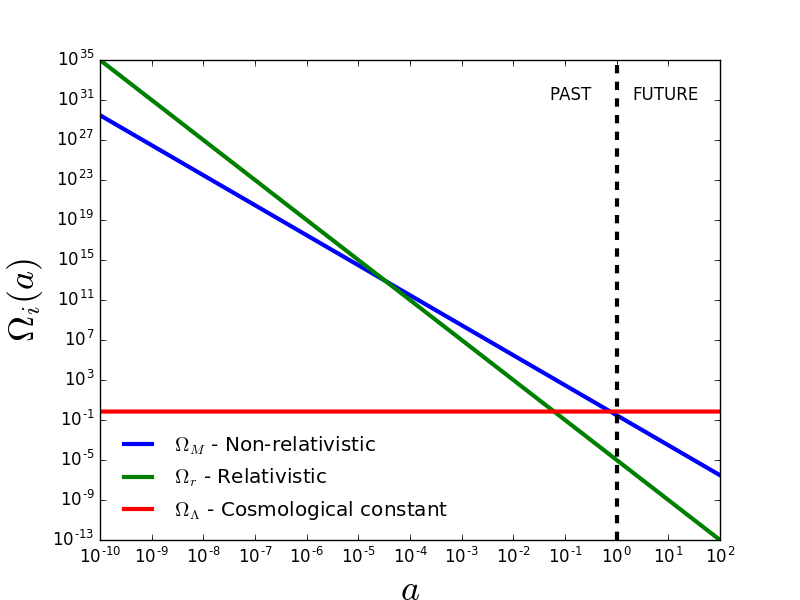
\includegraphics[width=0.85\textwidth]{./Pictures/rho_a.png}
\caption{Energy density for different types of matter species as function of the scale parameter of the Universe: relativistic (radiation) on green, non-relativistic (matter) on blue, and cosmological constant on red. It can be seen that at present (black-dashed line), cosmological constant has just started to be dominant over the other species.}
\label{fig:rho_de}
\vspace*{0.2cm}
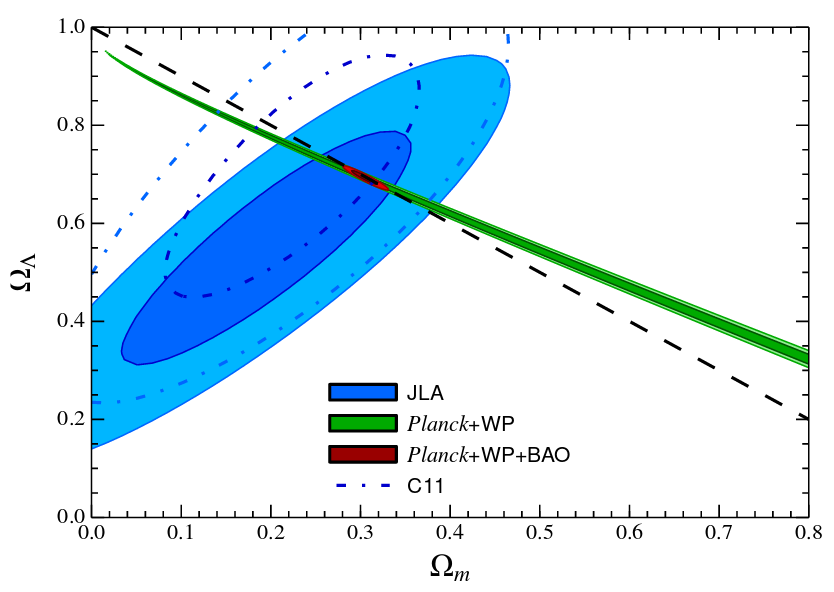
\includegraphics[width=0.8\textwidth]{./Pictures/om_ol.png}
\caption{Determination of the non-relativistic matter and dark energy content of the universe with the combination of SNIa, BAO, CMB. Image credit: \cite{2014A&A...568A..22B}.}
\label{fig:om_ol}
\end{center}
\end{figure}
\newline

General Relativity with the FLRW metric constitutes the theoretical basis for the current standard cosmological model: $\Lambda$CDM. It states that the Universe is flat, homogeneous and isotropic. The observational basis of $\Lambda$CDM are:
\begin{itemize}
\item {\bf The dark matter:} The presence of a new form of matter has been proposed to explain the measurement of the rotation curve of spiral galaxies \cite{1982ApJ...253...70B,1983Sci...220.1339R,1985ApJ...297..423B,1985ApJ...289...81R}. Dark matter is a form of matter that is not in the Standard Model of High Energy Physics and interacts with the ordinary --a.k.a. baryonic-- matter through gravity. Although several attempts have been made to constrain the nature of dark matter direct and indirectly, no evidence of its existence {\it in laboratories} has been found  \cite{2016JPhG...43a3001M,2016ConPh..57..496G}. On \autoref{fig:om_ol}, the determination of the energy density of dark energy and dark matter, assuming the $\Lambda$CDM model can be seen. Rotation curves and the large-scale-structure of the Universe agree mutually on the existence of dark matter.

\item {\bf The Cosmic Microwave Background (CMB):} The Cosmic Microwave background is the oldest light of the Universe that can be observed. It is composed by the photons that decoupled from baryons at redshift $z=1100$, when the Universe became colder and the energy of the photons was not enough to ionize hydrogen. The energy distribution of the CMB-photons corresponds to a black-body spectrum with temperature $T_{CMB}=2.72$ K. The spatial distribution of the temperature anisotropies is related to the physics of the interaction of the photons and can be divided in two types: primary --those produced by the interaction of the photons with the baryons at the last scattering surface-- and secondary --produced by the interaction of photons with the intergalactic medium and the gravitational potentials--. The power spectrum of the CMB anisotropies can be seen in \autoref{fig:cmbpk} with a fit to the $\Lambda$CDM cosmology. This excellent agreement on such a very wide range of scales is a major success for $\Lambda$CDM. In addition, the energy distribution of the CMB photons has a black-body spectrum, as predicted by $\Lambda$CDM.

\item {\bf The accelerated expansion of the Universe:} The expansion of the Universe was discovered by Hubble \cite{1929PNAS...15..168H}. Hubble established a linear relationship between the recession velocity of nearby galaxies which holds for low redshifts. Nevertheless, the improvement of the measurement with the inclusion of the data of the luminosity-distance relationship with type-Ia supernovae (SNIa) showed the accelerated expansion of the Universe \cite{1999ApJ...517..565P} (\autoref{fig:snlcdm}). The accelerated expansion of the Universe is translated on Einstein's field equation as a non-zero cosmological constant.

\item {\bf The baryon acoustic oscillations (BAO):} The baryon acoustic oscillations are produced in the early Universe, when matter and radiation are coupled. Anisotropies in the gravitational fields lead to the collapse of matter on the wells of the potential. This leads to an increase of the temperature on the regions with higher density due to the matter-radiation coupling. The increase of the temperature produces a positive pressure that ejects matter outside the potential wells. The matter collapse and the radiation pressure produce acoustic waves that at matter-radiation decoupling leave a characteristic scale --the BAO scale--. This translates on peak on the angular distribution of matter and constitutes an standard ruler to measure cosmological distances (\autoref{fig:baolcdm}).

\item {\bf The primordial nucleosynthesis:} The primordial nucleosynthesis or Big Bang nucleosynthesis is the production of the lightest elements of the periodic table other than hydrogen: deuterium, tritium, $^3$He, $^4$He, $^7$Li and $^7$Be. The production of heavier elements other than the mentioned is not possible since there are not stable elements with mass-number five or eight. The relative abundance of these elements is governed --in addition to the nuclear properties of the elements-- by the expansion of the Universe and the baryon-radiation ratio \cite{2006IJMPE..15....1S}.
\end{itemize}

\begin{figure}
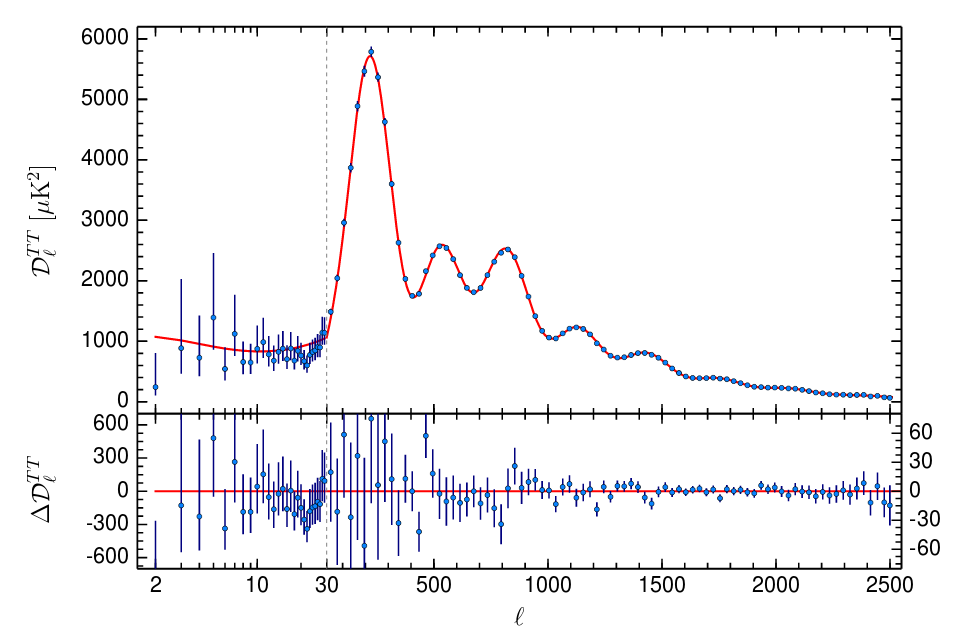
\includegraphics[width=\textwidth]{./Pictures/CMB_pk.png}
\caption{Power spectrum of the CMB. Red line is the best-fit to $\Lambda$CDM. Image credit: \cite{2015arXiv150201589P}}
\label{fig:cmbpk}
\end{figure}

\begin{figure}
\begin{center}
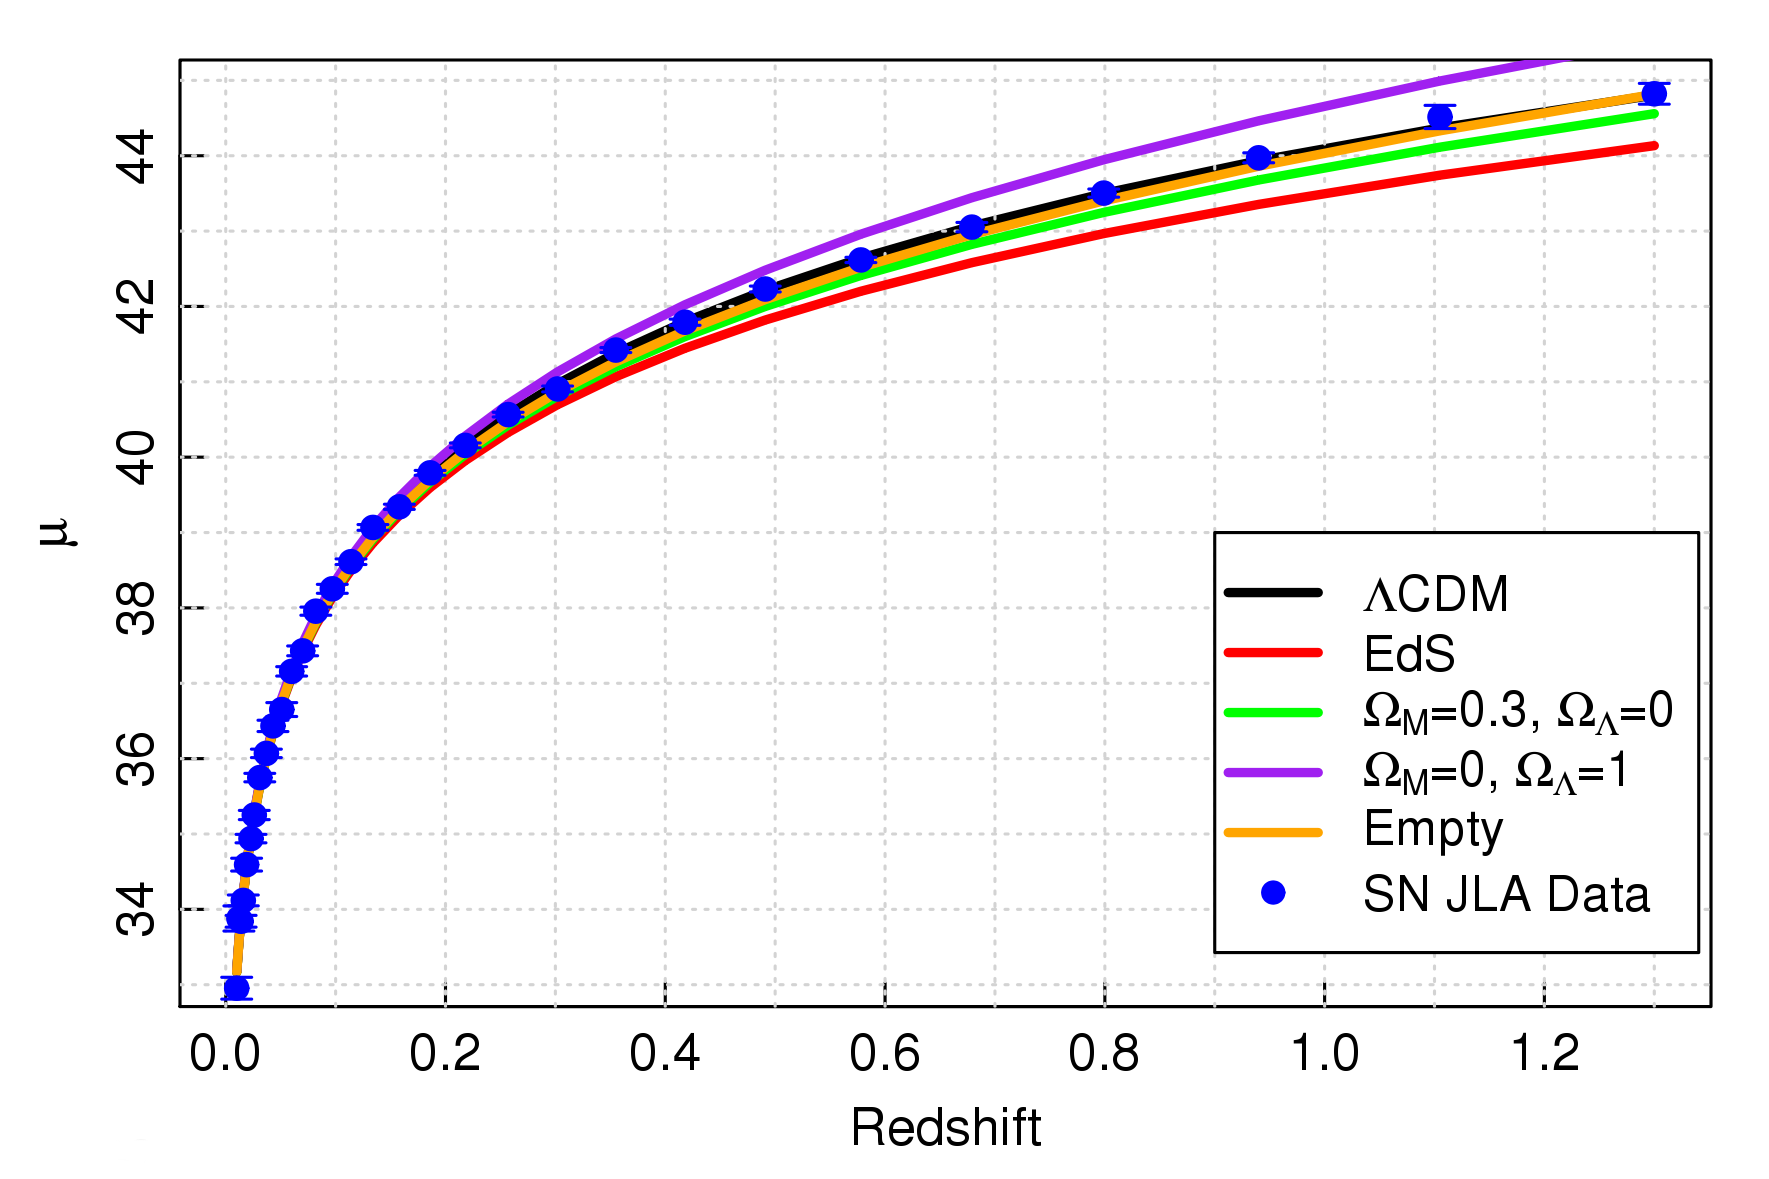
\includegraphics[width=1.0\textwidth]{./Pictures/distance_modulus.png}
\caption{Distance modulus measured by the JLA supernovae. Results are compared with different cosmological models based on General Relativity.}
\label{fig:snlcdm}
\vspace*{0.2cm}
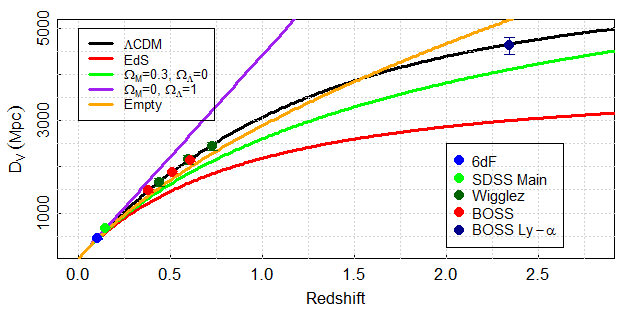
\includegraphics[width=1.0\textwidth]{./Pictures/bao_dv.png}
\caption{BAO distance-scale measured at different redshifts by different experiments. Results are compared with cosmological models based on General Relativity.}
\label{fig:baolcdm}
\end{center}
\end{figure}

\section{The Cosmological Constant problem}
The most general expression of Einstein's field equations contains the cosmological constant term, that can be absorbed on the right-hand-side of the \autoref{eq:einsteinbare} and interpreted as a constant matter term known as dark energy:
\begin{equation}
R_{\mu\nu}-\frac{1}{2}Rg_{\mu\nu} = \frac{8\pi G_N}{c^4}T_{\mu\nu}-\Lambda g_{\mu\nu}.
\end{equation}
With this matter term, assuming $\Omega_K=0$, \autoref{eq:flrw} transforms into
\begin{equation}
H^2(t) = H_0^2\left[\sum_i\Omega_i(t) +\Omega_\Lambda(t)\right],
\end{equation}
where $\Omega_\Lambda(t)=\Omega_\Lambda^0$ is the dark energy density. This new term is a time-independent constant that has the same value on every location of the Universe. Thus, while the other matter species have a density that decreases with time, the dark energy density is constant and becomes dominant at late cosmic times.
\newline

This new term may be regarded as a new matter species such that its energy density is given by
\begin{equation}
\rho_\Lambda = \frac{3H_0^2}{8\pi G_N}\Omega_\Lambda\sim 10 ^{-47} \mbox{ GeV}^4.
\label{eq:cosmologicalconstant}
\end{equation}
\newline

If $T_{\mu\nu}=0$ there is no matter/energy, the $\Lambda g_{\mu\nu}$ term acts as an alternative source of energy and can be identified as the vacuum energy density \cite{0038-5670-11-3-A13,RevModPhys.61.1,2003PhR...380..235P,PhysRevD.72.021301}. The dominant source for the vacuum energy within the Standard Model of Particle Physics is the Higgs field \cite{1974JETPL..19..183L,PhysRevLett.34.777}, a complex scalar-field that fills the Universe and gives mass to the elementary particles. The potential of the field is given by
\begin{equation}
V(\phi) = \mu_H^2\phi^\dagger\phi+\frac{1}{4}\lambda_H(\phi^\dagger\phi)^2,
\end{equation}
with $\mu_H$ the mass term, $\lambda_H$ the self-interaction of the field and $\phi,\phi^\dagger$ the Higgs field and its hermitian conjugate respectively. Thus, the cosmological constant can also be interpreted as the expected value of Higgs field \cite{1974JETPL..19..183L,PhysRevLett.34.777}
\begin{equation}
\langle 0|\phi_0|0\rangle = \frac{|\mu_H|}{\sqrt{\lambda_H}}= \sqrt{\frac{1}{\sqrt{2}G_F}}= 246\mbox{ GeV}^4,
\end{equation}
which shows a huge discrepancy with the cosmological constant energy density as given by \autoref{eq:cosmologicalconstant}. Here $G_F$ is the Fermi constant, that can be computed from the decay of the muon.

\section{Theories for Dark Energy}
As it has been stated previously, the observed value of the cosmological constant can not be explained with the Standard Model of High Energy Physics. Thus, one can try to explain accelerated expansion of the Universe with other class of theories. The simplest approach is to postulate the existence of new exotic fields with negative pressure that drive the accelerated expansion. The other possibility is an extension of General Relativity.

\subsection{Exotic matter fields}
A possible explanation to the accelerated expansion of the Universe can be found on the presence on new quantum fields. The simplest case is known as quintessence and is defined as a scalar field  ($\phi$) that is added to the action defined at \autoref{eq:ehaction} such that
\begin{equation}
S = \frac{c^4}{16\pi G_N}\int d^4x\sqrt{-g}R+S_\phi+S_M
\end{equation}
with
\begin{equation}
S_\phi = \int d^4x\left[\frac{1}{2}g^{\mu\nu}\partial_\mu\phi\partial_\nu\phi-V(\phi)\right],
\end{equation}
where $V(\phi)$ is the potential of the field. On the FLRW metric, this leads to a substance with pressure and density respectively 
\begin{equation}
P_\phi = \frac{1}{2}\dot\phi^2-V(\phi)\ \ \mbox{ and }\ \ \rho_\phi=\frac{1}{2}\dot\phi^2+V(\phi).
\end{equation}
This can be parametrized as an ideal fluid with equation of state
\begin{equation}
w_{DE} = \frac{P_\phi}{\rho_\phi} = \frac{\dot\phi^2-2V(\phi)}{\dot\phi^2+2V(\phi)}.
\end{equation}
Thus, it can be deduced that dark energy density evolves with the scale factor of the universe as
\begin{equation}
\Omega_\Lambda(t) = \Omega_\Lambda^0 [a(t)]^{-3(1+w_\phi)},
\end{equation}
if $w_\phi$ is constant.
\newline

This quintessence approach allows to explain any dark energy model by choosing properly the potential of the field. A detailed description of all the models can be found in \cite{2010deto.book.....A}. The most widely used phenomenological description is made in terms of the equation of state of dark energy,
\begin{equation}
P_{DE} = w_{DE}\rho_{DE}
\end{equation}
expanding the parameter $w_{DE}$ in a power series of the scale factor
\begin{equation}
w_{DE}(t) = w_0 +w_a[1-a(t)],
\end{equation}
where $w_0$ denotes the value of the equation of state parameter at present and $w_a$ its evolution --at first order-- with time. The cosmological constant may be considered as an specific solution of this equation of state where
\begin{equation}
w_0=-1\ \ \mbox{ and }\ \ w_a=0.
\end{equation}
The key difference between the cosmological constant and other exotic forms of matter is that the latter provide a dark energy density that evolves throughout cosmic history.

\subsection{Modified Gravity}
The other possibility to explain the accelerated expansion of the Universe is to assume that General Relativity is not valid at all cosmological distances and ages. Thus, data from cosmic expansion are not interpreted properly, requiring and extension of the theory.  Extensions to General Relativity are known as modified gravity models.
\newline

In order to preserve the symmetries of General Relativity, the new gravitational field equations must be a function of the Ricci scalar. The most general class of those theories is known as $f(R)$ gravity \cite{2010LRR....13....3D,2010RvMP...82..451S}, and its approach is to let the action be a general function ($f$) of the Ricci scalar:
\begin{equation}
S = \frac{c^4}{16\pi G_N}\int d^4x\sqrt{-g}f(R)+S_M,
\end{equation}
that leads to the field equation
\begin{equation}
R_{\mu\nu}-\frac{1}{2}Rg_{\mu\nu}=\frac{8\pi G_N}{c^4}( T_{\mu\nu}+T_{\mu\nu}^R).
\end{equation}
This field equation is similar to \autoref{eq:einsteinbare} but has an additional term $T_{\mu\nu}^R$ that takes into account the additional curvature terms that can be modeled as a fluid on the same way as the energy-momentum tensor. The simplest case is $f(R) =R+\alpha R^n$ with $\alpha,n\in\mathbb{R}$, which has interesting cosmological solutions \cite{PhysRevD.85.083511}. This theory has very distinctive phenomenology such as double Einstein rings with just one source galaxy on the strong lens regime \cite{2011PhRvD..83b4030N} that --if found--, could be the smoking gun of these kind of theories. The existence of a double Einstein ring (SDSSJ0946+1006) has been reported \cite{2008ApJ...677.1046G}, nevertheless it is a system with one lens and two sources at different redshifts, producing one ring of different diameter each.
\newline

More complicated models of modified gravity that may break the equivalence principle and the local Lorentz symmetry can be considered but are not going to be treated here. For a review the reference \cite{2015CQGra..32x3001B} can be consulted. The usual approach to explore the modifications to General Relativity \cite{2015PhRvD..91h3504L} is to consider the departures of the observed metric respect to General Relativity. On the Newtonian gauge, the FLRW line element can be parametrized with the Newtonian and the lensing potential; $\Phi,\Psi$ respectively \cite{2015PhRvD..91h3504L}:
\begin{equation}
ds^2 = a^2(\tau)[-(1+2\Psi)d\tau^2+(1-2\Phi)dx_idx^j],
\end{equation}
with
\begin{equation}
2\nabla^2\Phi(a,k) = \frac{8\pi G_N}{c^2}a^2\mu(a,k)\bar \rho_M\delta_M(a,k)\ \ \mbox{ and }\ \ \gamma(a,k)=\frac{\Phi(a,k)}{\Psi(a,k)},
\end{equation}
where $\bar \rho_M$ is the average matter density, $\delta_M$ its fluctuations and $k$ is the wavenumber of the potentials. Here $\mu$ and $\gamma$ parametrize the departures from General Relativity, that is the specific case with
\begin{equation}
\mu(a,k) = 1\ \ \mbox{ and }\ \ \gamma(a,k) = 1.
\end{equation}

\section{Current status of dark energy constrains}
The nature of dark energy can be constrained using different cosmological probes \cite{Weinberg201387} by measuring the $w_0,w_a$ parameters of its equation of state or the potentials $\Sigma,\gamma$ of modified gravity. There are two classes of cosmological probes: geometric and structure formation and evolution tests.
\newline

Geometrical measurements exploit the fact that the distances measured on cosmological scales depend on the metric tensor of the Universe, which is affected by its energy content and the assumed gravitational theory. These measurements include: the baryon acoustic oscillation peak-scale (BAO), the SNIa distance-ladder, Alcock-Paczynski \cite{1979Natur.281..358A} tests and the integrated Sachs-Wolfe (ISW) effect. On the other side, structure evolution probes are based on the measurement of the inhomogeneities of the matter density field at different moments of cosmic history, which depend on the matter/dark-energy ratio and gravitational theory used. They include: the cluster-count evolution with redshift, redshift-space-distortions (RSD), lensing and the cosmic microwave background (CMB).
\newline

The combination of different cosmological probes leads to more accurate measurements and at the same time it breaks degeneracies on the determination of the cosmological parameters \cite{2006A&A...448..831Y,Weinberg201387}.
\newline

The latest and more precise results constraining the cosmological parameters are provided by the Planck Collaboration 2015 results from the analysis of the Cosmic Microwave Background (CMB) \cite{2016A&A...594A..14P}, the recalibrated supernovae sample JLA \cite{2014A&A...568A..22B}, and the BAO scale-evolution with redshift by BOSS \cite{Ata:2017dya}, WiggleZ \cite{2014MNRAS.441.3524K}, SDSS \cite{2015MNRAS.449..835R} and 6dF \cite{2011MNRAS.416.3017B}.
\newline

Dark Enery as a new quantum field, is determined by measuring the parameters of the equation of state (see \autoref{fig:jlaw0}). Results are compatible with General Relativity plus cosmological constant, but the uncertainty on the parameters of the equation of state does not allow to exclude many models, since the current precision on the determination of the evolution parameter $w_a$ is still limited. Constrains on Modified Gravity models are also given in terms of the modified gravity potentials $\mu,\eta$ and $\Sigma$ (see \autoref{fig:mg_planck2015}).
\newline

\begin{figure}
\begin{center}
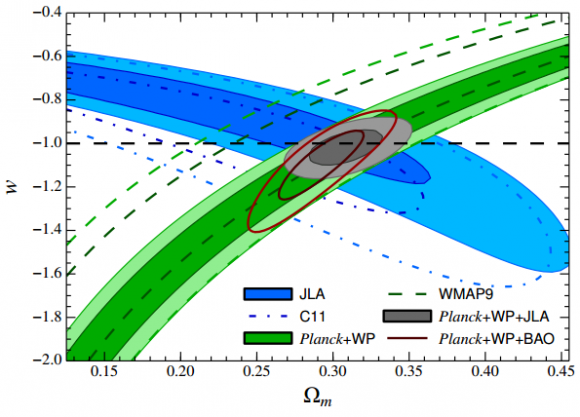
\includegraphics[width=0.8\textwidth]{./Pictures/JLA_w.png}
\caption{One- and two- sigma contours of the dark energy equation of state $w$ and matter content $\Omega_M$. Dashed line is General Relativity plus cosmological constant. Image credit: \cite{2014A&A...568A..22B}.}
\label{fig:jlaw0}
\vspace*{0.2cm}
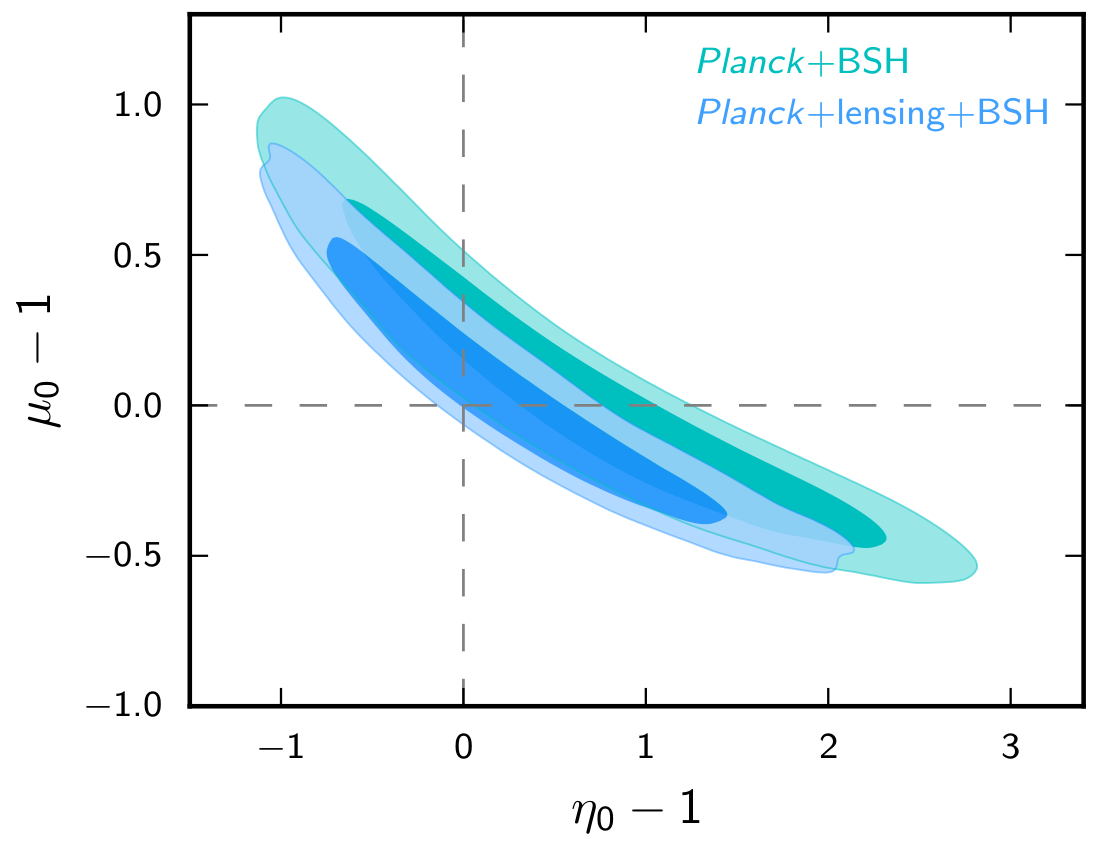
\includegraphics[width=0.8\textwidth]{./Pictures/mg_planck2015.png}
\caption{One- and two- sigma modified gravity potentials at present $\mu_0,\eta_0$. Dashed line is General Relativity plus cosmological constant. Image credit: \cite{2016A&A...594A..14P}.}
\label{fig:mg_planck2015}
\end{center}
\end{figure}
The latest results from the Sloan Digital Sky Survey (SDSS) and its upgrade BOSS, provide several measurements that show a good agreement with the $\Lambda$CDM paradigm. These probes include: Alcock-Paczynski tests \cite{2016ApJ...832..103L}, the clustering of galaxies \cite{2016arXiv160703155A}, baryon acoustic oscillations (BAO) \cite{2016arXiv160703154W,2017arXiv170200176B,Ata:2017dya} and redshift-space distortions \cite{2017MNRAS.465.1757G}.
\newline

Although several probes agree among them and seem to favour the cosmological constant as the origin of dark energy, there are some measurements that are in tension with Planck Collaboration 2015. Riess et~al. latest direct determination of the Hubble constant using the cosmological distance ladder (parallax-cepheids-SNIa) \cite{2016ApJ...826...56R}, show a discrepancy at the $3\sigma$ level with the Hubble constant measured by Planck Collaboration 2015. Weak-gravitational lensing  by CFHTLens and KiDS show tension with Planck Collaboration CMB measurements if a General Relativity plus cosmological constant scenario is considered \cite{2013MNRAS.430.2200K,2017arXiv170303383H,2017MNRAS.467.3024L}. This tension may be alleviated if other models are considered, such as non-zero curvature and dark energy models \cite{2016arXiv161004606J,2017arXiv170400762D,2017arXiv170108165Z}. Nevertheless, discrepancies can also be produced by systematic effects \cite{2015PhRvD..92b3003D,2017MNRAS.465.2033J}. At any case, the weak-lensing/CMB discrepancy is still not significant enough to put the $\Lambda$CDM model in crisis.
\newline

The current cosmological model --$\Lambda$CDM--, has demonstrated to be a solid theory that explains a wide range of physical effects and has passed the most stringent tests (\autoref{fig:cmbpk}, \autoref{fig:snlcdm} and \autoref{fig:baolcdm}). Although recent measurements show a small tension that may be alleviated in a  non-cosmological constant scenario, caution is needed and special attention is required to do a proper systematic error estimation. This requires additional probes and redundant measurements of the same physical observable but with different sources of systematic errors. We have entered in the precision cosmology era.

\section{Weak-lensing magnification as a probe for dark energy}
Weak-lensing magnification is produced by the same physical entity as the gg-lensing, but has lower signal-to-noise (see \autoref{ch:theory} for a full explanation of magnification and gg-lensing). Thus, the inclusion of magnification on a multiprobe analysis does not lead, generally, to a large improvement of the measurement. In order to achive this, we need to use magnification on environments and regimes that other probes can not reach. 
\newline

The strength of magnification is that it allows to measure directly the matter profile of the large-scale-structures that conform the Universe. The whole matter structures of the Universe are only accessible directly trough gravitational lensing due to the presence of dark matter. Since dark matter is not visible and interacts only through gravity, assumptions on how the visible- --baryonic- -- and dark- matter assemble together must be made on measurements other than gravitational lensing, introducing nuisance parameters.
\newline

A particular interesting system for weak-lensing measurements are voids. Since they have a lower matter content than the average Universe, their gravitational evolution is more dominated by dark energy. Thus, void properties depend on the nature of dark energy. If the abundance of large voids on the Universe is considered, it has been reported that its number increases in $f(R)$ gravity models \cite{2012MNRAS.421.3481L,2017JCAP...03..012V}. Nevertheless, if the shape of the void is measured, its ellipticity can be used as a probe for the parameters of the equation of state of dark energy \cite{2010MNRAS.403.1392L,0004-637X-754-2-109,PhysRevLett.98.081301,2013PhRvL.111x1103S}, since the structure growth-factor on the line-of-sight has a variation due to
the dark energy content, whereas on the transverse plane, growth-factor is constant. Finally, the radial distribution of matter around the center of a void --known as void profile-- has demonstrated to be different on $f(R)$ theories and General Relativity \cite{2014APh....54...44A,2014arXiv1410.8355C,2015MNRAS.451.4215Z,2015JCAP...08..028B,2016PhRvD..93j3522A,2016PhRvD..94j3524A}. Thus, by simply measuring the void matter profile, constrains on dark energy can be set. This implies that the direct determination of the matter profile of voids by weak-lensing magnification, constitutes a promising and independent new probe on dark energy.
\newline

This Thesis is devoted to the analysis of weak-lensing magnification using the Dark Energy Survey data. The analysis is carried out on two different data-sets of the mentioned experiment with two different goals each. The first analysis is carried out on the Science Verification data-set, aiming the detection of the magnification signal and the development of new techniques of systematic error mitigation. Once the magnification signal has been detected, a new analysis on the Year 1 data-release is made with the methodology that has been established previously. Year 1 analysis is qualitatively different since its goal is to measure the convergence profile of voids to use it as a probe for dark energy.
\newline

The next chapter (\autoref{ch:theory}), describes the general weak-lensing formalism and explains the magnification theory and its observational effects. The experiment where this Thesis has been developed --the Dark Energy Survey-- is briefly described on \autoref{ch:DES}. The core of this work is found on \autoref{ch:magnification}, where the analysis of the Science Verification data and the Year 1 data are described extensively, concluding on \autoref{ch:conclusions}.
